\documentclass[11pt,a4paper]{extarticle}
\usepackage{cmap}
\usepackage[utf8x]{inputenc}
\usepackage[T2A,T1]{fontenc}
\usepackage[hidelinks]{hyperref} 
\usepackage[russian,english]{babel}
\usepackage{listings,lstautogobble}
\usepackage{amsthm}
\usepackage{amsmath}
\usepackage{amsfonts}
\usepackage{amssymb}
\usepackage{xcolor,colortbl}
\usepackage{graphicx}
\usepackage{subcaption}
\usepackage{enumerate}
\usepackage{perpage}
\usepackage{subcaption}
\usepackage{fullpage}
\usepackage[nottoc,numbib]{tocbibind}
\usepackage[russian,english]{babel}

\definecolor{Gray}{gray}{0.95}
\definecolor{Red}{rgb}{0.80,0.5,0.5}
\definecolor{Green}{rgb}{0.6,0.8,0.6}

\definecolor{Gray}{gray}{0.95}
\definecolor{Black}{gray}{0.1}
\definecolor{Red}{rgb}{0.80,0.5,0.5}
\definecolor{Green}{rgb}{0.6,0.8,0.6}

\definecolor{codegray}{rgb}{0.5,0.5,0.5}
\definecolor{codepurple}{rgb}{0.58,0,0.82}
\definecolor{backcolour}{rgb}{0.95,0.95,0.92}

\newlength{\twosubht}
\newsavebox{\twosubbox}
\setlength\headheight{26pt}

\lstdefinestyle{codestyle}{
    backgroundcolor=\color{backcolour},   
    commentstyle=\color{Green},
    breakatwhitespace=false,         
    breaklines=true,                 
    captionpos=b,                    
    keepspaces=true,                 
    showspaces=false,                
    showstringspaces=false,
    showtabs=false,                  
    tabsize=2,
    autogobble=true,
    inputencoding=utf8x,
    extendedchars=\true
}

\lstset{style=codestyle}

\newenvironment{compactlist}{
\begin{list}{{$\bullet$}}{
\setlength\partopsep{0pt}
\setlength\parskip{0pt}
\setlength\parsep{0pt}
\setlength\topsep{0pt}
\setlength\itemsep{0pt}
}}{
\end{list}
}

\MakePerPage{footnote}

\begin{document}
\selectlanguage{russian}
\begin{titlepage}
	\begin{centering}
		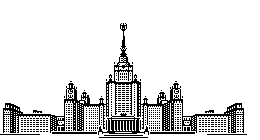
\includegraphics{img/msu}\\
		\large{
			\textbf{Московский государственный университет имени М.В. Ломоносова}\\
			Факультет вычислительной математики и кибернетики\\
			Кафедра интеллектуальных информационных технологий\\[4cm]
		}
		\Large{
			Гончаренко Дмитрий Александрович\\[0.9cm]
		}
		\Large{
			\textbf{Алгоритм изменения времени суток на изображении}\\
			% \textbf{Research of Changing The Time of Day on Images}\\
		}
		\rule[0.3cm]{14cm}{0.02cm}\\[1cm]
		\large{
			ВЫПУСКНАЯ КВАЛИФИКАЦИОННАЯ РАБОТА\\[4cm]
		}
	\end{centering}
	\begin{flushright}
		\large{
			\textbf{Научный руководитель:}\\ К.С. Зипа\\
		}
	\end{flushright}
	\begin{center}
		\vfill
		\large{
			Москва, 2019
		}
	\end{center}
\end{titlepage}

\begin{abstract}
	Алгоритм изменения времени суток на изображении относится к классу задач машинного обучения по \textit{переносу
	изображений}\footnote{
		\textbf{Перенос изображений} (англ. \textit{image translation}, или \textit{image transfering})
		-- подвид технологии переноса обучения, позволяющий сохранять и объединять локальные признаки изображений.
	}.
	Данная сфера значительное продвинулась благодаря современным вычислительным возможностям, в частности переносе обучения на графические процессоры, GPU.
	За последние несколько лет появилось немало исследовательских работ на тему переноса изображений, стилей и колоризации.
	В данной работе рассматриваются современные подходы к переносу изображений на примере изменения времени суток на изображении.
	Проводится описание нейросетевых моделей и сравнительный анализ серии экспериментов обучения.
\end{abstract}

\selectlanguage{english}
\begin{abstract}
	The algorithm of changing the time of the day on images is a subclass of Machine Learning problems of image translation.
	This area has advanced significantly due to the modern computing capabilities, in particular the training transfer on GPUs.
	Over the past few years, many research papers have appeared on the subject of images translation, styles transfering and colorization.
	This research reveals modern approaches of image translation on the example of changing the time of day on the image.
	A description of the neural network models and a comparative quality analysis of a series of training experiments are carried out.
\end{abstract}
\selectlanguage{russian}

\newpage
\tableofcontents
\newpage

\section{Введение}
	Математические описания моделей машинного обучения появились еще в середине 20-го века.
	А первые попытки их практической реализации начались в конце 50х годов.
	В наше время задачи машинного обучения все также не теряют своей актуальности.
	Рост числа работ, открытие исследовательских центров внутри компаний и при университетах показывает высокий интерес к данной сфере не только в науке.
	Появление удобных и современных инструментов для построения самых разнообразных моделей обучения,
	возможности мгновенно обмениваться информацией -- оказало немалое влияние на развитие \textit{науки о данных}\footnote{
		\textbf{Наука о данных} (англ. \textit{data science}) -- соовокупность процессов и методов направленных на извлечение информации из исследуемых данных.
	}.  
	
	Стоит отметить, что не последнюю роль здесь сыграли многократно выросшие вычислительные возможности. 
	Это позволило обучать \textit{нейронные сети}\footnote{
		\textbf{Нейронная сеть} --  математическая модель, а также её программное или аппаратное воплощение, 
		построенная по принципу организации и функционирования биологических нейронных сетей -- сетей нервных клеток живого организма.
		Является мощным современным инструментом машинного обучения.
		Главная особенность -- способность обучаться на предоставленных данных, называемых тренировочными.
		Помимо исследовательских направлений нейронные сети также активно используются в комерции, например обработка спама на электронной почте и система рекомендаций в интернет-магазинах.
	} на персональных компьютерах за доли секунды, для чего ранее могли требоваться дни, а то и недели на специализированных вычислительных устройствах.

	\textit{Перенос обучения} является одной из центральных исследовательских задач современного машинного обучения.
	Данная область направленна на получение некоторой информации об объекте, сохранение и последующее применение этих знаний к другому объекту, связанному с первым.   
	\textit{Перенос изображений}, в свою очередь, является подклассом переноса обучения применяемым на изображениях. 
	В настоящее время перенос изображений используется самыми разнообразными способами.
	С помощью него можно добиться объединения стилей двух изображений \cite{style_transfer},
	\textit{колоризации}\footnote{
		\textbf{Колоризация} (англ. \textit{colorization}) -- преобразование монохромных изображений в цветные.
	} черно-белых фотографий \cite{color_transfer}, объединение локальных признаков объектов и животных \cite{CycleGAN},
	увеличение разрешения изображений \cite{super_resolution}.

	В данной исследовательской работе рассматриваются и систематизируются современные подходы переноса изображений, на примере изменения времени суток на изображениях.
	А также проводится обучение моделей на различных наборах данных и сравнительный анализ полученных результатов с использованием предложенной метрики.
	
	В качестве инструмента был выбран фреймворк PyTorch\footnote{
		\textbf{PyTorch} -- библиотека машинного обучения, основанная на Torch. Разработана исследовательской группой в Facebook
	}, так как он разработан в виде библиотеки для языка Python - основного языка современного машинного обучения \cite{ml_lang},
	и зарекомендовал себя мощным и гибким инструментом для исследования и обучения нейронных сетей.

\newpage
\section{Постановка задачи}
	\subsection{Цель работы}
		В науке о данных одну из ключевых ролей играет непосредственный выбор данных, на которых будет обучаться сеть, 
		и которые будут использоваться для валидации качества модели. Перенос изображений не является исключением.
		Цель работы -- получить модель, которая будет уметь с высокой точностью переносить изображения между \textit{доменами}\footnote{
			\textbf{Домен} -- область, множество, содержащее в себе объекты одного типа. 
		} и способную решить проблему изменения времени суток на изображениях с приемлемой точностью.
	
	\subsection{Решаемые задачи}
		Проблему изменения времени суток на изображении можно разбить на следующие этапы:

		\begin{itemize}
			\item Исследование существующих методов переноса изображений и решений родственных задач
			\item Поиск применимых к проблеме тренировочных данных -- изображений с различными временами суток, и их применение
			\item На основе проведенного исследования и обзора литературы, выбрать модель, наилучшим образом подходящую,
			для решения поставленной задачи
			\item Множественное обучение выбранной модели на различных конфигурациях с помощью библиотеки PyTorch
			\item Разработка и применение метрики качества обучения для выявления наилучших параметров сети
			\item Проведение серии экспериментов для получения оценки качества и скорости работы модели 
		\end{itemize}

	\subsection{Формальная постановка задачи}
		Формально алгоритм изменения времени суток на изображении можно сформулировать следующим образом:

		\subsubsection*{Вход}
			На вход алгоритму поступают два изображения из различных доменов \(x_{1} \in X_{1}\)  и \(x_{2}\ \in X_{2}\), где
			\begin{itemize}
				\item \(X_{1}\) -- домен с набором изображений первого типа
				\item \(X_{2}\) -- домен с набором изображений второго типа
			\end{itemize}
			Не ограничивая общности пусть \(X_{1}\) соодержит изображения дня, а \(X_{2}\) соответвует ночи.
		\subsubsection*{Выход}
			Необходимо произвести \textit{кросдоменные переносы}\footnote{
				\textbf{Кросдоменный перенос} (англ. \textit{cross-domain transfer}) -- перенос объектов между доменами 
			}: \(x_{1} \rightarrow x_{2} \) (сменить время суток на изображении со дня на ночь)
			и \(x_{2} \rightarrow x_{1} \) (с ночи на день)
			
			\noindent
			% \begin{center}
			\begin{equation}
				x_{1}  = CrossDomainModel(x_{2}) \\
				x_{2}  = CrossDomainModel(x_{1})
			\end{equation}
				% \end{center}
	% \section{Предметная область}
% \section{Обзор существующих решений рассматриваемой задачи}

% \section{Исследование и построение решения задачи}

% \section{Описание практической части}
% \textit{датасетов}\footnote{
% 				\textbf{Датасет} (англ. \textit{dataset}) -- то же, что и набор данных.
% 				} 
% \section{Заключение}

\newpage

\begin{thebibliography}{00}

	\bibitem{style_transfer}
	\textbf{J.Johnson, A.Alahi, L.Fei-Fei}.
	\emph{Perceptual Losses for Real-Time Style Transfer and Super-Resolution}.
	Department of Computer Science, Stanford University,
	March 2016.

	\bibitem{color_transfer}
	\textbf{R.Zhang, J.-Y.Zhu, P.Isola, X.Geng, A.S.Lin, T.Yu, A.A.Efros}.
	\emph{Real-Time User-Guided Image Colorization with Learned Deep Priors}.
	University of California, Berkeley,
	May 2017.

	\bibitem{CycleGAN}
	\textbf{J.-Y.Zhu, T.Park, P.Isola, A.A.Efros}.
	\emph{Unpaired Image-to-Image Translation using Cycle-Consistent Adversarial Networks}.
	Berkeley AI Research (BAIR) laboratory, UC Berkeley,
	November 2018.

	\bibitem{super_resolution}
	\textbf{Y.Yuan, S.Liu, J.Zhang, Y.Zhang, C.Dong, L.Lin}
	\emph{Unsupervised Image Super-Resolution using Cycle-in-Cycle Generative Adversarial Networks}
	Guangdong Key Laboratory of Intelligent Information Processing, Shenzhen University,
	Graduate School at Shenzhen, Department of Automation, Tsinghua University,
	September 2018.

	\bibitem{UNIT}
	\textbf{M.-Y.Liu, T.Breuel, J.Kautz}.
	\emph{Unsupervised Image-to-Image Translation Networks}.
	NVIDIA Corporation,
	Jule 2018.
	
	\bibitem{MUNIT}
	\textbf{X.Huang, M.-Y.Liu, S.Belongie, J.Kautz}.
	\emph{Multimodal Unsupervised Image-to-Image Translation}.
	Cornell University, NVIDIA Corporation,
	August 2018.

	\bibitem{BicycleGAN}
	\textbf{J.-Y.Zhu, R.Zhang, D.Pathak, A.A.Efros}.
	\emph{Toward Multimodal Image-to-Image Translation}.
	Berkeley AI Research, UC Berkeley, Adobe Research,
	October 2018.

	\bibitem{EG-UNIT}
	\textbf{L.Ma, X.Jia, S.Georgoulis, T.Tuytelaars, L.V.Gool}.
	\emph{Exemplar Guided Unsupervised Image-to-Image Translation}.
	Berkeley AI Research, UC Berkeley, Adobe Research,
	March 2019.
	
	\bibitem{Deep_Learning}
	\textbf{С.Николенко, А.Кадурин, Е.Архангельская}.
	\emph{Глубокое обучение}.
	СПб.: Питер, 
	2018.

	\bibitem{ml_lang}
	\textbf{The State of the Octoverse: machine learning} --
	\href{https://github.blog/2019-01-24-the-state-of-the-octoverse-machine-learning/}{GitHub: Report},
	January 2019

\end{thebibliography}

\end{document}